

\tikzset{every picture/.style={line width=0.75pt}} %set default line width to 0.75pt        

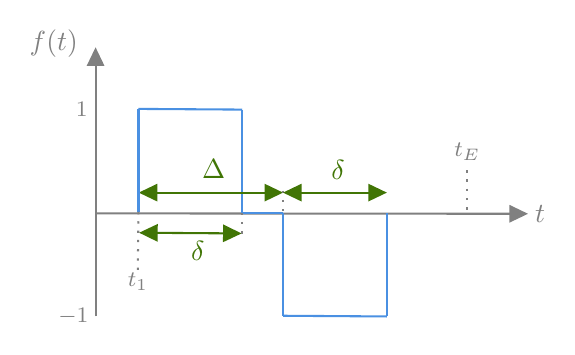
\begin{tikzpicture}[x=0.75pt,y=0.75pt,yscale=-1,xscale=1]
%uncomment if require: \path (0,300); %set diagram left start at 0, and has height of 300

%Straight Lines [id:da8882796881399757] 
\draw [color={rgb, 255:red, 128; green, 128; blue, 128 }  ,draw opacity=1 ]   (70.67,219.67) -- (70.67,93) ;
\draw [shift={(70.67,90)}, rotate = 90] [fill={rgb, 255:red, 128; green, 128; blue, 128 }  ,fill opacity=1 ][line width=0.08]  [draw opacity=0] (8.93,-4.29) -- (0,0) -- (8.93,4.29) -- cycle    ;
%Straight Lines [id:da664635011077519] 
\draw [color={rgb, 255:red, 128; green, 128; blue, 128 }  ,draw opacity=1 ]   (70.67,170) -- (276,170.2) ;
\draw [shift={(279,170.2)}, rotate = 180.06] [fill={rgb, 255:red, 128; green, 128; blue, 128 }  ,fill opacity=1 ][line width=0.08]  [draw opacity=0] (8.93,-4.29) -- (0,0) -- (8.93,4.29) -- cycle    ;
%Straight Lines [id:da17789798284277847] 
\draw [color={rgb, 255:red, 74; green, 144; blue, 226 }  ,draw opacity=1 ]   (91.33,119.67) -- (141.33,120) ;
%Straight Lines [id:da7626646796988461] 
\draw [color={rgb, 255:red, 74; green, 144; blue, 226 }  ,draw opacity=1 ]   (141.33,120) -- (141.33,169.67) ;
%Straight Lines [id:da4344394785262813] 
\draw [color={rgb, 255:red, 74; green, 144; blue, 226 }  ,draw opacity=1 ]   (141.33,169.67) -- (161,169.67) ;
%Straight Lines [id:da9282561195936812] 
\draw [color={rgb, 255:red, 74; green, 144; blue, 226 }  ,draw opacity=1 ]   (161,169.67) -- (161,219.33) ;
%Straight Lines [id:da08552867507313566] 
\draw [color={rgb, 255:red, 74; green, 144; blue, 226 }  ,draw opacity=1 ]   (161,219.33) -- (211,219.67) ;
%Straight Lines [id:da3575819731609853] 
\draw [color={rgb, 255:red, 74; green, 144; blue, 226 }  ,draw opacity=1 ]   (211,170) -- (211,219.67) ;
%Straight Lines [id:da12257132095246326] 
\draw [color={rgb, 255:red, 65; green, 117; blue, 5 }  ,draw opacity=1 ]   (94.67,179.35) -- (138,179.65) ;
\draw [shift={(141,179.67)}, rotate = 180.39] [fill={rgb, 255:red, 65; green, 117; blue, 5 }  ,fill opacity=1 ][line width=0.08]  [draw opacity=0] (8.93,-4.29) -- (0,0) -- (8.93,4.29) -- cycle    ;
\draw [shift={(91.67,179.33)}, rotate = 0.39] [fill={rgb, 255:red, 65; green, 117; blue, 5 }  ,fill opacity=1 ][line width=0.08]  [draw opacity=0] (8.93,-4.29) -- (0,0) -- (8.93,4.29) -- cycle    ;
%Straight Lines [id:da6443721529726347] 
\draw [color={rgb, 255:red, 65; green, 117; blue, 5 }  ,draw opacity=1 ]   (94.5,160) -- (158,160) ;
\draw [shift={(161,160)}, rotate = 180] [fill={rgb, 255:red, 65; green, 117; blue, 5 }  ,fill opacity=1 ][line width=0.08]  [draw opacity=0] (8.93,-4.29) -- (0,0) -- (8.93,4.29) -- cycle    ;
\draw [shift={(91.5,160)}, rotate = 0] [fill={rgb, 255:red, 65; green, 117; blue, 5 }  ,fill opacity=1 ][line width=0.08]  [draw opacity=0] (8.93,-4.29) -- (0,0) -- (8.93,4.29) -- cycle    ;
%Straight Lines [id:da43765182650583845] 
\draw [color={rgb, 255:red, 128; green, 128; blue, 128 }  ,draw opacity=1 ] [dash pattern={on 0.84pt off 2.51pt}]  (141.33,169.67) -- (141.33,180.33) ;
%Straight Lines [id:da9970970110276676] 
\draw [color={rgb, 255:red, 128; green, 128; blue, 128 }  ,draw opacity=1 ] [dash pattern={on 0.84pt off 2.51pt}]  (161,159) -- (161,169.67) ;
%Straight Lines [id:da9873905246267041] 
\draw [color={rgb, 255:red, 65; green, 117; blue, 5 }  ,draw opacity=1 ]   (164,160) -- (208,160) ;
\draw [shift={(211,160)}, rotate = 180] [fill={rgb, 255:red, 65; green, 117; blue, 5 }  ,fill opacity=1 ][line width=0.08]  [draw opacity=0] (8.93,-4.29) -- (0,0) -- (8.93,4.29) -- cycle    ;
\draw [shift={(161,160)}, rotate = 0] [fill={rgb, 255:red, 65; green, 117; blue, 5 }  ,fill opacity=1 ][line width=0.08]  [draw opacity=0] (8.93,-4.29) -- (0,0) -- (8.93,4.29) -- cycle    ;
%Straight Lines [id:da6590571773579443] 
\draw [color={rgb, 255:red, 128; green, 128; blue, 128 }  ,draw opacity=1 ] [dash pattern={on 0.84pt off 2.51pt}]  (249.73,149.2) -- (249.73,169.53) ;
%Straight Lines [id:da76362319772591] 
\draw [color={rgb, 255:red, 74; green, 144; blue, 226 }  ,draw opacity=1 ]   (91.33,119.67) -- (91.33,169.33) ;
%Straight Lines [id:da9036000522736403] 
\draw [color={rgb, 255:red, 128; green, 128; blue, 128 }  ,draw opacity=1 ] [dash pattern={on 0.84pt off 2.51pt}]  (91.33,169.33) -- (91,198.67) ;

% Text Node
\draw (63.6,88.2) node [anchor=east] [inner sep=0.75pt]  [color={rgb, 255:red, 128; green, 128; blue, 128 }  ,opacity=1 ]  {$f( t)$};
% Text Node
\draw (281,170.2) node [anchor=west] [inner sep=0.75pt]  [color={rgb, 255:red, 128; green, 128; blue, 128 }  ,opacity=1 ]  {$t$};
% Text Node
\draw (119.89,181.73) node [anchor=north] [inner sep=0.75pt]  [color={rgb, 255:red, 128; green, 128; blue, 128 }  ,opacity=1 ]  {$\textcolor[rgb]{0.25,0.46,0.02}{\delta }$};
% Text Node
\draw (127.55,142.4) node [anchor=north] [inner sep=0.75pt]  [color={rgb, 255:red, 128; green, 128; blue, 128 }  ,opacity=1 ]  {$\textcolor[rgb]{0.25,0.46,0.02}{\Delta }$};
% Text Node
\draw (187.55,154.99) node [anchor=south] [inner sep=0.75pt]  [color={rgb, 255:red, 128; green, 128; blue, 128 }  ,opacity=1 ]  {$\textcolor[rgb]{0.25,0.46,0.02}{\delta }$};
% Text Node
\draw (68.33,119.67) node [anchor=east] [inner sep=0.75pt]  [font=\footnotesize,color={rgb, 255:red, 128; green, 128; blue, 128 }  ,opacity=1 ]  {$1$};
% Text Node
\draw (68.67,219.67) node [anchor=east] [inner sep=0.75pt]  [font=\footnotesize,color={rgb, 255:red, 128; green, 128; blue, 128 }  ,opacity=1 ]  {$-1$};
% Text Node
\draw (91,197.4) node [anchor=north] [inner sep=0.75pt]  [font=\footnotesize,color={rgb, 255:red, 128; green, 128; blue, 128 }  ,opacity=1 ]  {$t_{1}$};
% Text Node
\draw (249.73,145.8) node [anchor=south] [inner sep=0.75pt]  [font=\footnotesize,color={rgb, 255:red, 128; green, 128; blue, 128 }  ,opacity=1 ]  {$t_{E}$};


\end{tikzpicture}
